\hfill
\setlength\parindent{5em}
\begin{minipage}{0.42\textwidth}
	
	\vspace{4em}
	{\LARGE \textbf{Квадрат Пирсона}}\\
	\vspace{1em}\\
	\textit{А.П. Азия, И.М. Вольпер}
	\vspace{5em}\\
В ''Занимательной алгебре'' Я. И. Перельмана есть любопытная задача под названием ''В парикмахерской''. В этой задаче автор рассказывает, что, заглянув однажды в парикмахерскую, он увидел, как мастера пытались безуспешно приготовить 12-процентный раствор перекиси водорода из двух имевшихся в наличии растворов \textemdash  трех- и тридцатипроцентного *).
\let\thefootnote\relax\footnotetext{ 
	*) Напомним, что содержанием вещества\\
	в растворе нахывается отношение массы\\
	этого вещества в ''чистом виде'' к массе\\
	раствора.} 
\\ \hspace*{\parindent} Задача, описанная Перельманом, встречается не только в парикмахерских.
\\ \hspace*{\parindent} Например, для зарядки аккумуляторов бывает необходимо приготовить электролит, который должен содержать 24\% серной кислоты из двух растворов с содержанием 92\% и 10\% серной кислоты. На консервных заводах возникает необходимость приготовления 6\%-ного уксуса для маринада из двух партий уксуса разной крепости: 3\% и 10\%, и т. д.
\\ \hspace*{\parindent} Для решения подобных задач удобно пользоваться ''квадратом Пирсона''. Вот как это делается. Рисуют квадрат и проводят две диагонали (рис. 1). В левом верхнем углу проставляют больший показатель крепости исходных веществ (\textit{а}), а в нижнем углу второй показатель (\textit{b}), а на пересечении диагоналей записывают требуемый показатель смеси (\textit{c}). Затем производят вычитание по первой диагонали (\textit{а - c}) и находят коли- 

\end{minipage}
\hfill
\begin{minipage}{0.48\textwidth}

чество второй части смеси (\textit{y}). Из центра производят вычитание по второй диагонали (\textit{с - b}) и находят количество первой части смеси (\textit{x}). Значения х и у записывают по одной линии с показателями. На х частей первого вещества надо взять у частей второго вещества, тогда получится смесь с по казателем \textit{с}.

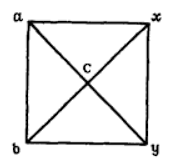
\includegraphics[width=0.48\linewidth]{Photo1.png}
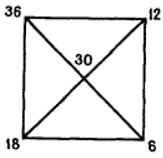
\includegraphics[width=0.44\linewidth]{Photo2.png}
\textbf{\quad Рис. 1. \qquad\qquad\qquad\quad Рис. 2.}


Пусть, например, имеются две партии сливок: одна содержит 36\% жира, а другая - 18\%. Требуется определить, сколько надо взять тех и других сливок, чтобы получить смесь с количеством жира 30\%. Решаем по изложенному выше способу (рис. 2) и получаем

\begin{center}
	$y=a - c = 36 - 30 = 6$\\
	$x = c - b = 30 - 18 = 12$
\end{center}



то есть на 6 массовых частей второй партии сливок надо взять 12 частей первой. 
\\ \hspace*{\parindent} Этот способ основан на специфи- \\ческом виде количества получаемой смеси, оно равно разности показате- лей исходных веществ. Такое допу- щение вполне возможно, так как нас интересуют не абсолютные величины, а относительные количества двух чаcтей смеси.
\\ \hspace*{\parindent} В самомеле, Мы получаем

\begin{center}
$x + y = (c - b) + (a + c) = a - b$
\end{center}

частей смеси. «Чистого» вещества в ней будет


$\qquad\frac{x \cdot a}{100} + \frac{y \cdot b}{100} = \frac{(c-b)a + (a-c)b}{100} = \frac{ac-bc}{100}$,
\\

частей, а крепость смеси будет равна\\

$\frac{ac-bc}{100(a-b)} = \frac{c}{100}$, то есть \textit{c}\%

\end{minipage}
\begin{flushright}\textbf{61}\end{flushright}
